\begin{figure*}[hbtp]
  \centering
  \subfigure[Initial graph]{
    \label{fig:about-frontier-01}
    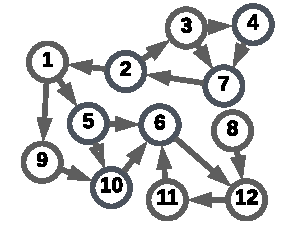
\includegraphics[width=0.23\linewidth]{out/about-frontier-01.pdf}
  }
  \subfigure[Marking affected (initial)]{
    \label{fig:about-frontier-02}
    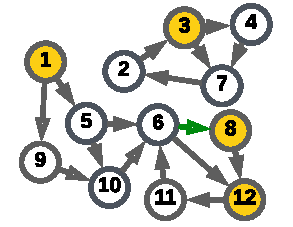
\includegraphics[width=0.23\linewidth]{out/about-frontier-02.pdf}
  }
  \subfigure[After first iteration]{
    \label{fig:about-frontier-03}
    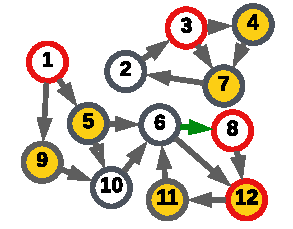
\includegraphics[width=0.23\linewidth]{out/about-frontier-03.pdf}
  }
  \subfigure[After second iteration]{
    \label{fig:about-frontier-04}
    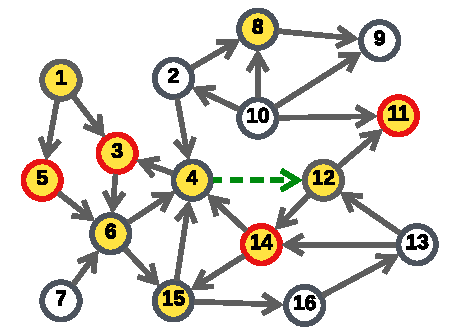
\includegraphics[width=0.23\linewidth]{out/about-frontier-04.pdf}
  } \\[-2ex]
  % \subfigure[]{
  %   \label{fig:about-frontier-05}
  %   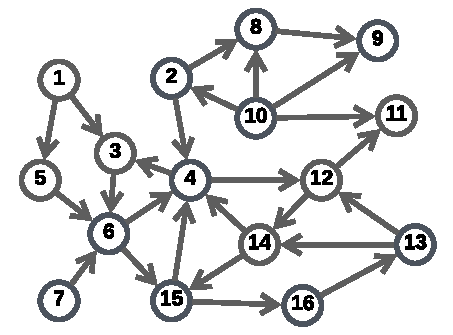
\includegraphics[width=0.18\linewidth]{out/about-frontier-05.pdf}
  % }
  \caption{Illustration of the \textit{Dynamic Frontier} approach through a specific example. The initial graph consists of $16$ vertices and $25$ edges. The graph is then updated with an edge insertion $(4, 12)$, and an edge deletion $(2, 1)$. Accordingly, the outgoing neighbors of vertices $4$ ($3$ and $12$) and $2$ ($1$, $4$, and $8$) are marked as affected (shown with yellow fill). When the ranks of these affected vertices are computed in the first iteration, it is found that change in rank of vertices $1$ and $12$ exceeds the frontier tolerance $\tau_f$ (shown with red border). Thus, outgoing neighbors of vertices $1$ ($3$ and $5$) and $12$ ($11$ and $14$) are also marked as affected. In the second iteration, the change in rank of vertices $3$, $5$, $11$, and $14$ is greater than $\tau_f$ --- thus their outgoing vertices are marked as affected. In the subsequent iteration, the ranks of affected vertices are again updated. If the change in rank of every vertex is within iteration tolerance $\tau$, the ranks of vertices have converged, and the algorithm terminates.}
  \label{fig:about-frontier}
\end{figure*}
